\documentclass{article}
\usepackage{hyperref}
\usepackage{graphicx}
\usepackage{amsmath}
\usepackage[a4paper, total={7.4in, 10in}]{geometry}

\begin{titlepage}
  \title{Report Third Project IAJ}
  \author{João Vítor ist199246
  \and Sebastião Carvalho ist199326
  \and Tiago Antunes ist199331}
  \date{2023-11-2}
\end{titlepage}

\begin{document}
  \maketitle
  \tableofcontents
  \newpage
  \section{Introduction}
  The goal of the project was to change the game of the second project, and implement a Reinforcement Learning algorithm to play it.\\
  For this, we first started with making the game restart when the player dies or wins the game, so that we can leave the agent to train
  without having to restart the simulation each time.\\
  We only implemented one Reinforcement Learning Algorithm: Q-Learning.\\
  \section{Game Changes and new States}
  \subsection{Game Changes}
  As said before, to make the game restart when the player dies or wins, we had to change certain aspects of the game.\\
  First, we started by not destroying the objects like chests and enemies when they were collected or killed. Instead, we just disabled 
  them by setting their active boolean to false. When the game ended, we simply changed all the objects' active flag back to true.
  We also created a restart function for NPCs, so that their base stats would go back to their initial stats. This is extremely useful for Sir Uthgard,
  to recover his health, level, etc., and for the enemies, so that they would respawn in their initial positions.\\
  We also created a new Script for collectable items like the potions and the chests, because sometimes the player would collide with them, 
  changing their position, and we needed this position to reset back whenever the game restarted.
  \subsection{New States}
  Since we decided to use Q-Learning, we also needed to change how we represented the state, since too many different states would make our 
  Q-Table too big and need a lot of memory. So, we decided to create another state representation, with less states, but still enough to 
  distinguish between different situations.\\
  We decided to use macro states, which are states that represent the current game state in a more simplified way, reducing the total number of possible states.
  The representation we chose varied across the development, so we decided to describe each one in the next section.
  \section{Q-Learning}
  \subsection{Algorithm}
  Q-Learning is a Reinforcement Learning algorithm, this means that occasionally the agent has rewards or punishments as a result of
  performing actions.\\
  For this algorithm we use macro states, these represent the current game state in a more simplified way, reducing the total
  number of possible states for the game. Anything that is not encoded in these states cannot be learned, so these changed as
  we improved the algorithm. For each state, the algorithm must also know what actions are available to it. This is because the
  algorithm will keep a Q Table that stores the quality of an action given a certain state, this is called the Q value.

  \[Q(s,a) = (1-\alpha)Q(s, a) + \alpha(r + \gamma * max(Q(s', a'))) \text{, $\alpha$ $\in$ [0,1], $\gamma$ $\in$ [0,1]}\]

  \noindent
  Where $s$ is the current state, $a$ is the action performed, $r$ is the direct reward for the performed action,
  $s'$ is the new state and $a'$ is the best action in the new state.\\
  $\alpha$ and $\gamma$ are the learning parameters.
  $\alpha$ is the learning rate and represents how much the new Q value will change because of the new reward.
  $\gamma$ is how much the indirect reward will propagate backwards.\\
  We kept $\alpha$ at 0.5 and $\gamma$ at 0.1 throught all iterations.
  \noindent
  After every execution of an action in a state, we update it's respective Q value acording to the formula above. 
  For our exploration strategy, we choose $\epsilon$-greedy, this means that for learning we get the action with the highest Q value for
  the state, most of the time, but we have a low chance of using a random action, $\epsilon$.\\
  
  \subsection{Training process}
  For the training process, we let the algorithm first run and calculate the Q values.
  We would then see the amount of victories and determine if we should let it run for longer. If the version seemed to be learning very little
  we cut the learning short but in other cases we let it run for about 1000 iterations.
  We would also note what the agent did in the run, to see if there was any any information
  in the state that he was missing.\\
  After this we would change what we thought was necessary and train the agent again. All enemy behavior was kept on during training.

  \section{Q-Learning Versions}
  \subsection{1st Version}
  For our states, we started by capturing what we felt was most important while still keeping the total amount of states as low as possible.
  We captured the characters' health, money, level, position and the time of the game.\\
  These stats were simplified in the following way.\\

  \subsubsection{States}
  \begin{table}[h!]
      \parbox{.45\linewidth}{
        \centering
        \caption{Simplified states of Health}
        \label{tab:tableA*1}
        \begin{tabular}{c|c}
          \textbf{Status} & \textbf{Health + Shield (interval)}\\
          \hline
          VeryLow & [0,6]\\
          Low & [7,12]\\
          OK & [13,18]\\
          Good & [19,30]\\
        \end{tabular}
      }
      \hfil
      \parbox{.45\linewidth}{
        \centering
        \caption{Simplified states of Time}
        \label{tab:tableA*2}
        \begin{tabular}{c|c}
          \textbf{Status} & \textbf{Time (interval)}\\
          \hline
          Early  & [0,49]\\
          Mid & [50,99]\\
          Late & [100,150]\\
        \end{tabular}
      }
  \end{table}
  \begin{table}[h!]
    \parbox{.45\linewidth}{
      \centering
      \caption{Simplified states of Money}
      \label{tab:tableA*3}
      \begin{tabular}{c|c}
        \textbf{Status} & \textbf{Money}\\
        \hline
        Poor & 0 and 5\\
        Mid & 10 and 15\\
        Rich & 20\\
      \end{tabular}
    }
    \hfil
    \parbox{.45\linewidth}{
      \centering
      \caption{Simplified states of Level}
      \label{tab:tableA*4}
      \begin{tabular}{c|c}
        \textbf{Status} & \textbf{Level}\\
        \hline
        Level2 & 2\\
        NotLevel2 & 1 and 3\\
      \end{tabular}
    }
  \end{table}
  \begin{table}[h!]
    \centering
    \caption{Simplified states of Position}
    \label{tab:tableA*5}
    \begin{tabular}{c|c|c}
      \textbf{Status} & \textbf{x Coordinates} & \textbf{z Coordinates}\\
      \hline
      TopLeft & $<=$ 66 & $>=$ 48.27\\
      TopRight & $>$ 66 & $>=$ 48.27\\
      BottomLeft & $<=$ 66 & $<$ 48.27\\
      BottomRight & $>$ 66 & $<$ 48.27\\
    \end{tabular}
  \end{table}
  \noindent
  This gave us a total amount of 288 possible states.\\
  The reason as to why we choose these divisions was due to our previous experiences with the game.\\
  Health is divided into intervals of 6 because that's the attack damage of the orcs, VeryLow will result in death if the
  character is attacked by an orc. We found these values to be descriptive enough that we
  didn't need to do intervals for the skeletons' damage.\\
  In terms of Time we considered 3 intervals. We simply considered that having 3 phases of the game was enough for Sir Uthgard to understand when it was more urgent to get the chests.\\
  For money, we gave it 3 states, we represent each 2 values in a state essencially. We did this in the hopes that the agent wouldn't need these intermediate values to learn that he should pick up the chests.\\
  Level only has 2 states, this is because out of observation we can see that it is possible to win only by being in level 2, and we don't want
  to waste any more time than we need leveling up or killing enemies.\\
  The last statistic is position, in here we divided the level into rectangles, this was done by analyzing the map and seeing what areas where more
  connected so that the character would prefer actions in one area.\\

  \subsubsection{Reward Function}

  Our initial reward function only rewarded the agent for reaching the win condition, in which case the reward was 100, or any of the loss conditions,
  where the reward was -100, as well as +0.1 for any state that was Level2.\\

  \subsubsection{Learning Parameters}

  We used $\alpha$ at 0.5 and $\gamma$ at 0.1, like specified before. The random action chance, $\epsilon$, was 5\%.\\

  \subsubsection{Results}

  In 400 iterations Sir Uthgard hadn't learnt much and won 0 times.\\
  With so few rewards, the algorithm didn't have enough guidance, and our whole approach to rewards was wrong. 
  We had to reward executing an action in a certain state, and not reward the states themselves. To do this, we had to consider the state we were in, and the state the action led to. 
  This also meant death and win states were useless, we simply had to reward the action.\\

  \subsection{2nd Version}

  \subsubsection{Improvements}

  In this second version we kept the same states. We focused mainly on improving the reward function.
  We rewarded +10 for going up a money state, +10 for actions that made a VeryLow hp state go to Good, +20 for leveling up. 
  Actions that made Uthgard change the quadrant of the map he was on were penalized with -1.

  \subsubsection{Results}

  Sir Uthgard displayed a much more intelligent behavior, and we saw him get his first win. After 252 runs, he had 168 deaths, 83 timeouts, and 1 win. 
  But unfortunately, after 2749 iterations, he had only won 15 times. The algorithm was still lacking direction, got stuck trying bad actions for too long and kept goofing around in the late game.

  \subsection{3rd Version}

  \subsubsection{Improvements}

  We increased the number of money states from 3 to 5: VeryPoor, Poor, Mid, Rich, and VeryRich. 
  
  \begin{table}[h!]
    \centering
    \caption{New simplified states of Money}
    \label{tab:tableA*6}
    \begin{tabular}{c|c}
      \textbf{Status} & \textbf{Money}\\
      \hline
      VeryPoor & 0\\
      Poor & 5\\
      Mid & 10\\
      Rich &  15\\
      VeryRich & 20\\
    \end{tabular}
  \end{table}
  \noindent
  This way, Uthgard would always be instantly rewarded for picking up a chest. This increased the number of states to 480. \\
  For the reward funtion, we added a -5 reward for actions in a Late game state that didn't lead to an increase in money. And we increased epsilon to 0.1, so he'd try new things more often.

  \subsubsection{Results}

  These changes were very effective. After 1013 runs, he had 666 deaths, 319 timeouts, and 28 wins. This is when we started to notice the biggest challenge to using Q learning for this problem. 
  Actions were getting mislabeled as bad. If Uthgard got killed or timed out while walking to a chest, picking up the chest would get a negative reward. 
  Sometimes, this was a good thing, for example, when he decided to pick up the chest on the bottom left as his first move. But would be very bad late game, as Uthgard was too scared to pick up the last chests.

  \subsection{4th Version}

  \subsubsection{Improvements}

  To avoid Sir Uthgard getting spooked of chests due to the timeouts, we removed the negative reward for timeouts all together. The action itself wasn't responsible for the loss, it was the combination of all actions that led to that point.  
  
  \subsubsection{Results}

  The change didn't have the impact we expected. The behavior was looking better, but the results were slightly worse. In 1005 iterations, he died 770 times, timed out 224, and won 11. We were still seeing the same problem.

  \subsection{5th Version}

  \subsubsection{Improvements}
  
  In the late game, since Sir Uthgard was often killed by the bottom left orc or by the dragon while going for those chests. He started doing everything except picking them up, even if those enemies were dead.
  So, we added a new variable to the state. DragonAndOrc: EitherAlive if at least one was alive, and BothDead. This would help him understand that the chests weren't scary if those enemies weren't there. 

  \begin{table}[h!]
    \centering
    \caption{States for Dragon and bottom left Orc}
    \label{tab:tableA*7}
    \begin{tabular}{c|c|c}
      \textbf{Status} & \textbf{Dragon} & \textbf{Botton Left Orc}\\
      \hline
      EitherAlive & Alive & Alive\\
      EitherAlive & Alive & Dead\\
      EitherAlive & Dead & Alive\\
      BothDead & Dead & Dead\\
    \end{tabular}
  \end{table}
  \noindent
  Theoretically, this would increase the number of states to 960, but, since most of the time one of them was alive, there wouldn't be that many more states in practice. 
  We also added a +10 reward for transitioning to a state where they were both dead.

  \subsubsection{Results}

  Now, in 1001 runs, he had 691 deaths, 264 timeouts, and 46 wins. At this point, putting epsilon at 0, Uthgard won 15/20 runs. And after arduous over-night training with an epsilon of 0.1, and some extra runs with epsilon at 0 to refine his strategy, he had a 20/20 win rate. 
  4585 runs, 2279 deaths, 1776 timeouts, and 530 wins later, Uthgard had learnt how to clear the dungeon. But we were still not satisfied.

  \subsection{6th Version}

  \subsubsection{Improvements}

  For this version, we wanted him to learn faster, in a more stable way and win in less time.\\
  We tried increasing the reward for picking up chest to +15. We decreased the penalty for actions that didn't lead to an increase in money in the late game to -4 and changed how it worked. Previously, if Uthgard was attacked by an orc while going for a chest, picking it up would get a -5 rewarded because the state would be updated, and the action had not led to more money. 
  Now, we made it so picking up chest actions can't get this penalty. We made the transition from Low hp to Good hp also get a +10 reward, instead of only VeryLow to Good. We changed Late to start at 90 seconds. And finally, the win reward is now +100 + [time remaining], to incentivize faster runs.

  \subsubsection{Results}

  This didn't lead to him learning faster. After more than 4000 iterations with an epsilon of 0.1, he had won less times. The difference wasn't significant enough not to be blamed on luck, but also didn't improve the learning timewise in any noticeable way.
  However, he seemed a lot more stable as we started to have him run without random actions. Within less runs than previously, he had 100\% win rate in 141 runs. And won, on average, 20 seconds faster than before. At the end, the algorithm had run 4781 times, with 2885 deaths, 1441 timeouts and 455 wins. The Q table saw 403 states.

  \section{Final Version of Q-Learning}

  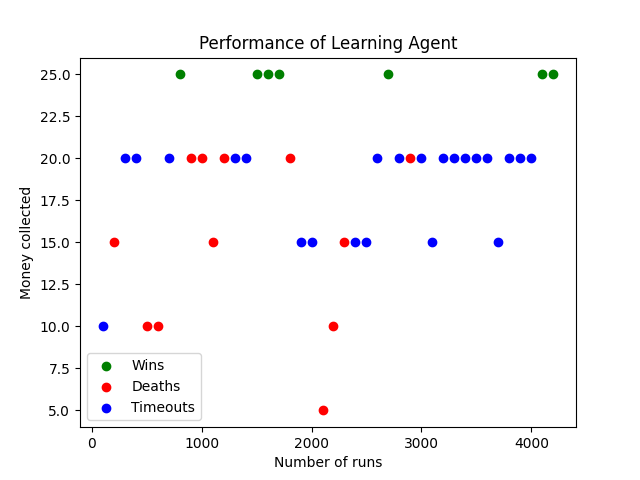
\includegraphics{graph.png}

  \section{Conclusions}
  

\end{document}
